\section{Space as Resource}
Space plays a vital role in advancing science, technology, and the broader progress of humanity. Through the exploration of space, scientists gain unique insights into the origins of the universe, the behavior of physical laws under extreme conditions, and the potential for life beyond Earth. Technological developments driven by space missions — from satellite communications to materials engineering — often find critical applications on Earth, improving everyday life and driving innovation across industries. Beyond the tangible benefits, space exploration inspires a sense of curiosity, unity, and ambition, encouraging humanity to transcend borders and collaborate on solving challenges that face us collectively. As we expand our presence beyond Earth, space becomes not only a frontier of discovery but also a catalyst for technological and social progress on a global scale.

% The space industry drives innovation across a wide range of sectors, from communications and navigation to climate monitoring and national security. By investing in space technologies, we enable new economic opportunities, support critical infrastructure on Earth, and open pathways for future exploration beyond our planet. As the industry grows, it fosters collaboration, inspires technological breakthroughs, and strengthens the resilience of modern society.

% primary areas are earth observaion, communications and positioning/timing.

\section{Space as a Manufacturing Environment}
The appeal of in-space manufacturing is not only the reduction in cost, ... and ... for goods used on Earth, it is also the number of possibilities that become available due to a diverse and mobile manufacturing base that can support [megastructures and stuff].

Microgravity, vacuum and abundant solar energy are all inherent to the space environment but very expensive to achieve on earth. This means any products with either of these requirements of the manufacturing process are dramatically cheeper to manufacture in space.

Microgravity and nanotubes and stuff


Vacuum and pure material science and stuff


Solar heating or cooling for free
% The potential for in-space manufacturing is a game-changer for the future of space exploration and industry. By enabling the production of components and materials in space, we can reduce reliance on Earth-based supply chains, minimize launch costs, and enhance mission flexibility. In-space manufacturing opens up new possibilities for building habitats, spacecraft, and other structures directly in orbit or on celestial bodies, paving the way for sustainable human presence beyond Earth. This capability not only supports long-duration missions but also fosters innovation in materials science and engineering, ultimately transforming our approach to space exploration and resource utilization.
% In space manufacturing overcomes many of the limitations of traditional manufacturing. The microgravity environment allows for unique material properties and processes that are not achievable on Earth. This can lead to the development of advanced materials, improved manufacturing techniques, and the ability to create complex structures that are lightweight and strong. Additionally, the vacuum of space allows for the production of high-purity materials, which can be critical for certain applications, such as electronics or optics. The vacuum also enables cost-compettitve temperature extremes due to the lack of conduction and convection. In earths orbit, satellites facing the sun can heat surfaces to over 1000k [cite] or allow them to cool down to 100k [cite] in the eclipse. Finally, manufacturing in space can avoid the need to design around violent launch loads, usually not experienced in the satellites operational environment. This allows for the design of more complex and capable systems, which can be critical for certain applications, such as space telescopes or planetary landers. Overall, in-space manufacturing has the potential to revolutionize the way we build and operate spacecraft, making them more efficient, cost-effective, and capable of meeting the challenges of future technology.
\newpage
\section{Additive Manufacturing}
Additive manufacturing (AM), also known as 3D printing, is a transformative technology that enables the layer-by-layer construction of complex structures from stock material. This approach is particularly well suited to space manufacturing due to its significantly lower material waste, high design flexibility, and the ease of transporting raw materials such as filament or powder. Prefabricated components like I-beams or plates can impose strict constraints on launch vehicle payload dimensions. Whereas raw materials for additive manufacturing are compact, lightweight, and adaptable to a wide range of mission needs.

For structural components of any space mission, the requirements to be compact enough to fit into the payload fairing and strong enough to withstand the launch vibrations sacrifice [efficiency and reliability wantt o get across big optimisation problem]. If these parts are manufactured once they are in orbit, the designs can be tailored to the orbital manoeuvre loads alone, increasing mission flexibility. 

Additionally, the crucial benefit of additive manufacturing is its ability to repair and modify existing components. This capability is especially valuable in space, where repairs can be challenging and costly. By enabling on-demand production of spare parts or modifications to existing systems, additive manufacturing enhances the resilience and longevity of space missions, reducing the need for extensive inventories of spare parts and minimizing the risk of mission failure due to component obsolescence or damage.
\section{Previous work}
This FYP is a continuation of the COSMOS project looking at additive manufacturing in space using cold spray. Cold spray was found to be the most promising area of research [cite from other guy] because of its high rate of deposition and independence from the microgravity environment.

Experiments have since been conducted using a full cold spray system in a vacuum chamber. While the experiments were a success they could have been improved in x y z ways.

\newpage

\section{Objectives}

The previous design of the powder feed tank, seen in \autoref{fig:current-feed-system-exploded-diagram}, resembled a typical fluidized powder bed used in the chemical engineering industry. The gas flows from bottom to top and, given a high enough flow rate, entrains the particles into the flow.
\begin{figure}[htbp]
    \centering

    \begin{minipage}{0.3\textwidth}
        \centering
        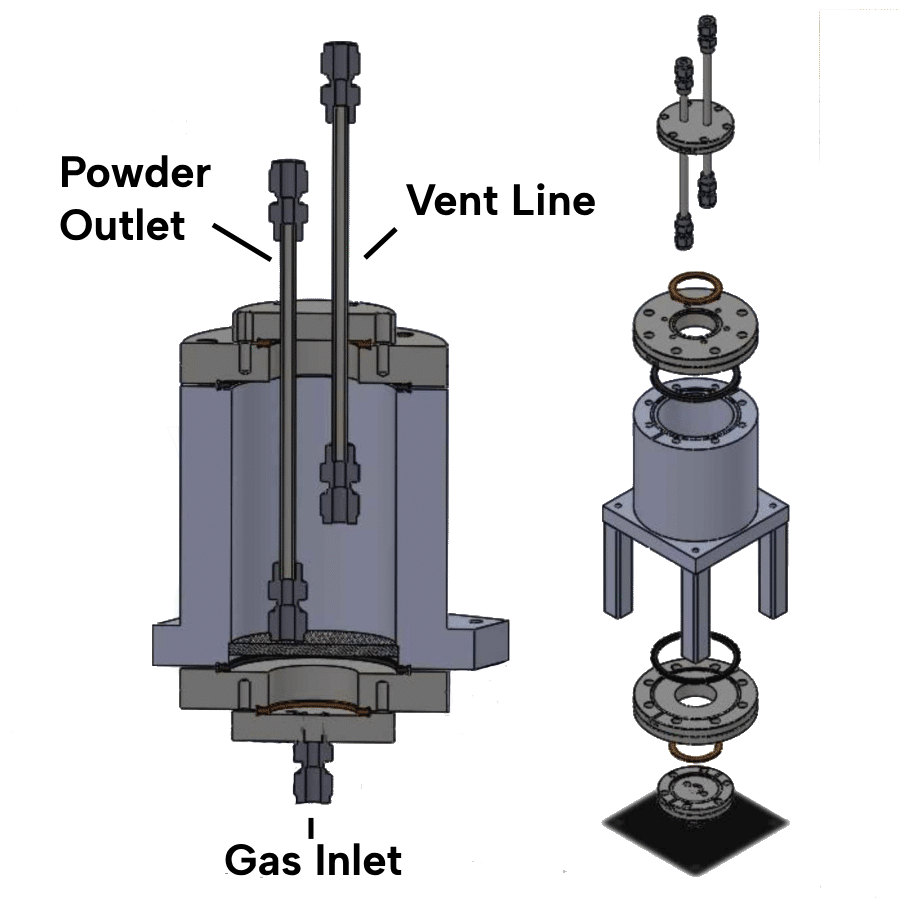
\includegraphics[width=\textwidth]{../report_assets/COSMOS_DIAGRAM.png}
        \caption{Current feed system diagram.}\label{fig:current-feed-system-exploded-diagram}
    \end{minipage}
    \hfill
    \begin{minipage}{0.3\textwidth}
        \centering
        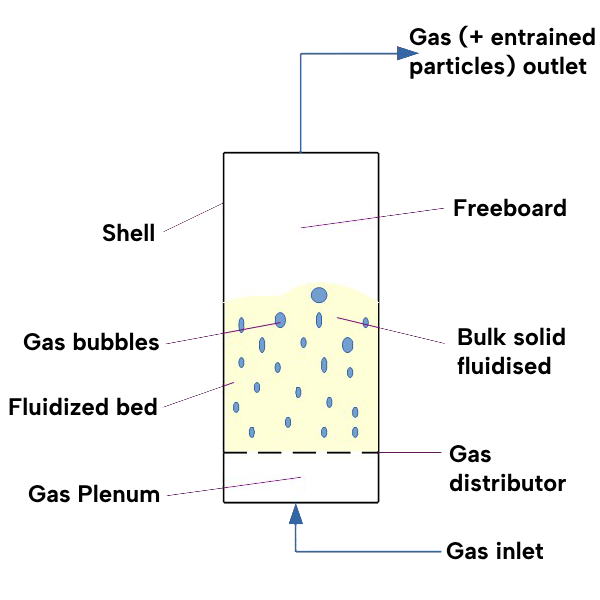
\includegraphics[width=\textwidth]{../report_assets/Fluidized_Bed_polished.png}
        \caption{Simplified fluidized powder bed diagram.}\label{fig:fluidized-bed-diagram}
    \end{minipage}
    \hfill
    \begin{minipage}{0.3\textwidth}
        \centering
        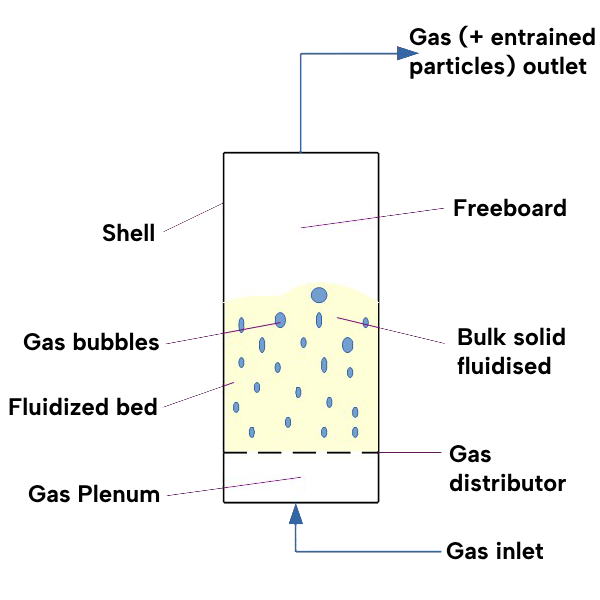
\includegraphics[width=\textwidth]{../report_assets/Fluidized_Bed_polished.png}
        \caption{Current design with turbulent inlet.}\label{fig:current-feed-system-fluent}
    \end{minipage}

\end{figure}

This design was suitable enough to facilitate the testing of the cold spray system in a vacuum chamber, but it would not be capable of operating under microgravity conditions. This is because the powder, that would sit on top of the mesh, is not being held at this location. Meaning that the powder is free to float away from the outlet and prevent the system from functioning. This was verified through 2 phase fluent simulations shown in figure \autoref{fig:current-feed-system-fluent}. 
% Further investigations, seen in \autoref{fig:current-feed-system-fluent-turbulent} into whether a turbulent inlet could mix the powder in the tank yielded the same results. 
% Therefore, to increase the fidelity of the experiment, the system needed to be redesigned to account for this.

Additionally, there is no mechanism to control the mass flow rate of the powder. This is a key parameter in the cold spray process, as it directly affects the critical velocity of the particles and in turn the porocity of the deposition. 


Finally, typical to any space mission, mass must be kept to a minimum and reliability is of the upmost importance. Maybe talk about redundancy implementations in the design here?
Therefore, the goals of the new design are to:
\begin{itemize}
    \item Constrain the powder to the inlet of the system
    \item Design for controlability of the mass flow rate
    \item Prioritise low mass and high reliability
\end{itemize}
